\chapter{Extrinsic Calibration}
\label{chapter:extrinsic_calibration}

In order to combine cameras together in one visual SLAM framework, extrinsic calibration between all cameras needs to be performed.  This means finding a transformation that can transform data from one camera's frame to another.  It is critical that such a calibration is highly accurate i.e. well within 0.1$^{\circ}$.  Even a very small rotational offset will result in a significant reprojection error when reprojecting points from one camera to another.  Take for example a rotational error of 0.5$^{\circ}$.  Over a distance of 10m, this would result in a reprojection error of 8.7 pixels for a standard digital camera.

\section{Extrinsic calibration tool}
\label{sec:ros_tool}
%TODO: understand this better

An extrinsic calibration between multiple perspective cameras can be performed given a checkerboard of known dimensions.  If the checkerboard is visible and can be detected from all cameras, a non linear optimization to determine the 6 DoF transformation between cameras can be performed.  A tool to provide such functionality is provided as a ROS package.\footnote{Camera pose calibration, \url{http://wiki.ros.org/camera_pose_calibration?distro=groovy}}  This package was utilised in order to obtain an initial estimate of the transformation from stereo to omni camera.

\begin{figure}[h!]
  \centering
    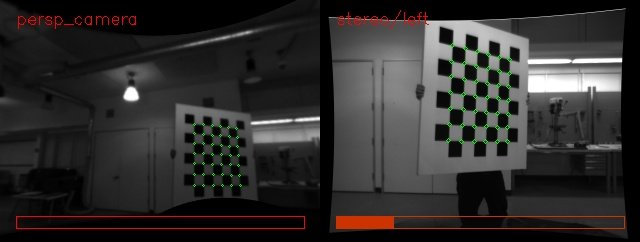
\includegraphics[width=1.0\textwidth]{chapters/images/extrinsic_cal_1}
  \caption{Extrinsic calibration tool provided by ROS}
  \label{fig:extrinsic_cal_1}
\end{figure}

\section{Omni Camera Perspective Image}
\label{sec:perspective_from_donut}
%TODO fix citaion
The package as described above for the extrinsic calibration works only for perspective cameras. This means cameras for which the intrinsic parameters are known and images are undistorted such that all straight lines appear straight.  However this is not the case for the omni camera.  Both the original donut image and unwrapped circular image are distorted and therefore will not work with the camera pose calibration package.  Therefore a new camera projection for the omni cam is necessary, to represent part of the omni image as a perspective type projection.

An algorithm was developed to create a perspective image for calibration from the unwrapped image.  Using Scaramuzza's camera model\cite{scaramuzza_06} there exists a  mapping from 3D ray to pixel coordinates, and pixel coordinates to 3D ray.  Given these functions it is possible to create a perspective image, what is required is a set of 3D rays to be defined for every pixel of the perspective image.  The algorithm for creating 3D rays and populating the perspective image is as follows:

\begin{algorithm}[h!]
 \caption{Algorithm to generate perspective image}
 %\SetLine % For v3.9
 %\SetAlgoLined % For previous releases [?]
 Initialize $\bv I(cols,rows)$; \ \ \ \ \ \ \ \ \ \ \ \ \ \ \ \ \ \ \ \ \ \ \ \ \ \ \ \ \ 
 // perspective image to populate \\
 $u_c = cols/2$;  \\
 $v_c = rows/2$;  \\
 Define $\bv F_{ray}$; \ \ \ \ \ 
 // vector that points to center of desired perspective image \\
 $\bv F_{ray} = \bv F_{ray}.normalize()$ * focal length; \ \ \ \ \ \ \ \ \ \ \ \ \ \ \ \ \\
 %// set $\norm {\bv F_{ray}} $ to focal length \\
 Define $\bv u$ and $\bv v$; \ \ \ \ \ \ \ \ 
 //vectors orthogonal to $\bv F_{ray}$ that define image plane \\
 $\bv u$.normalize(); \\
 $\bv v$.normalize(); \\
 \For{v = 0 to rows}
 {
   $\bv v_{ray}$ = $\bv v \times (v - v_c)$; \\
   \For{u = 0 to cols}
   {
     $\bv u_{ray}$ = $\bv u \times (u - u_c)$; \\
     $\bv P_{ray} = \bv F_{ray} + \bv u_{ray} + \bv v_{ray}$; \\
     $\bv P_{img}$ = project($\bv P_{ray})$; \\
     $\bv I(u,v)$ = bilinearInterpolate($\bv P_{img}$)
   }
 }
\end{algorithm}

\begin{figure}[h!]
  \centering
    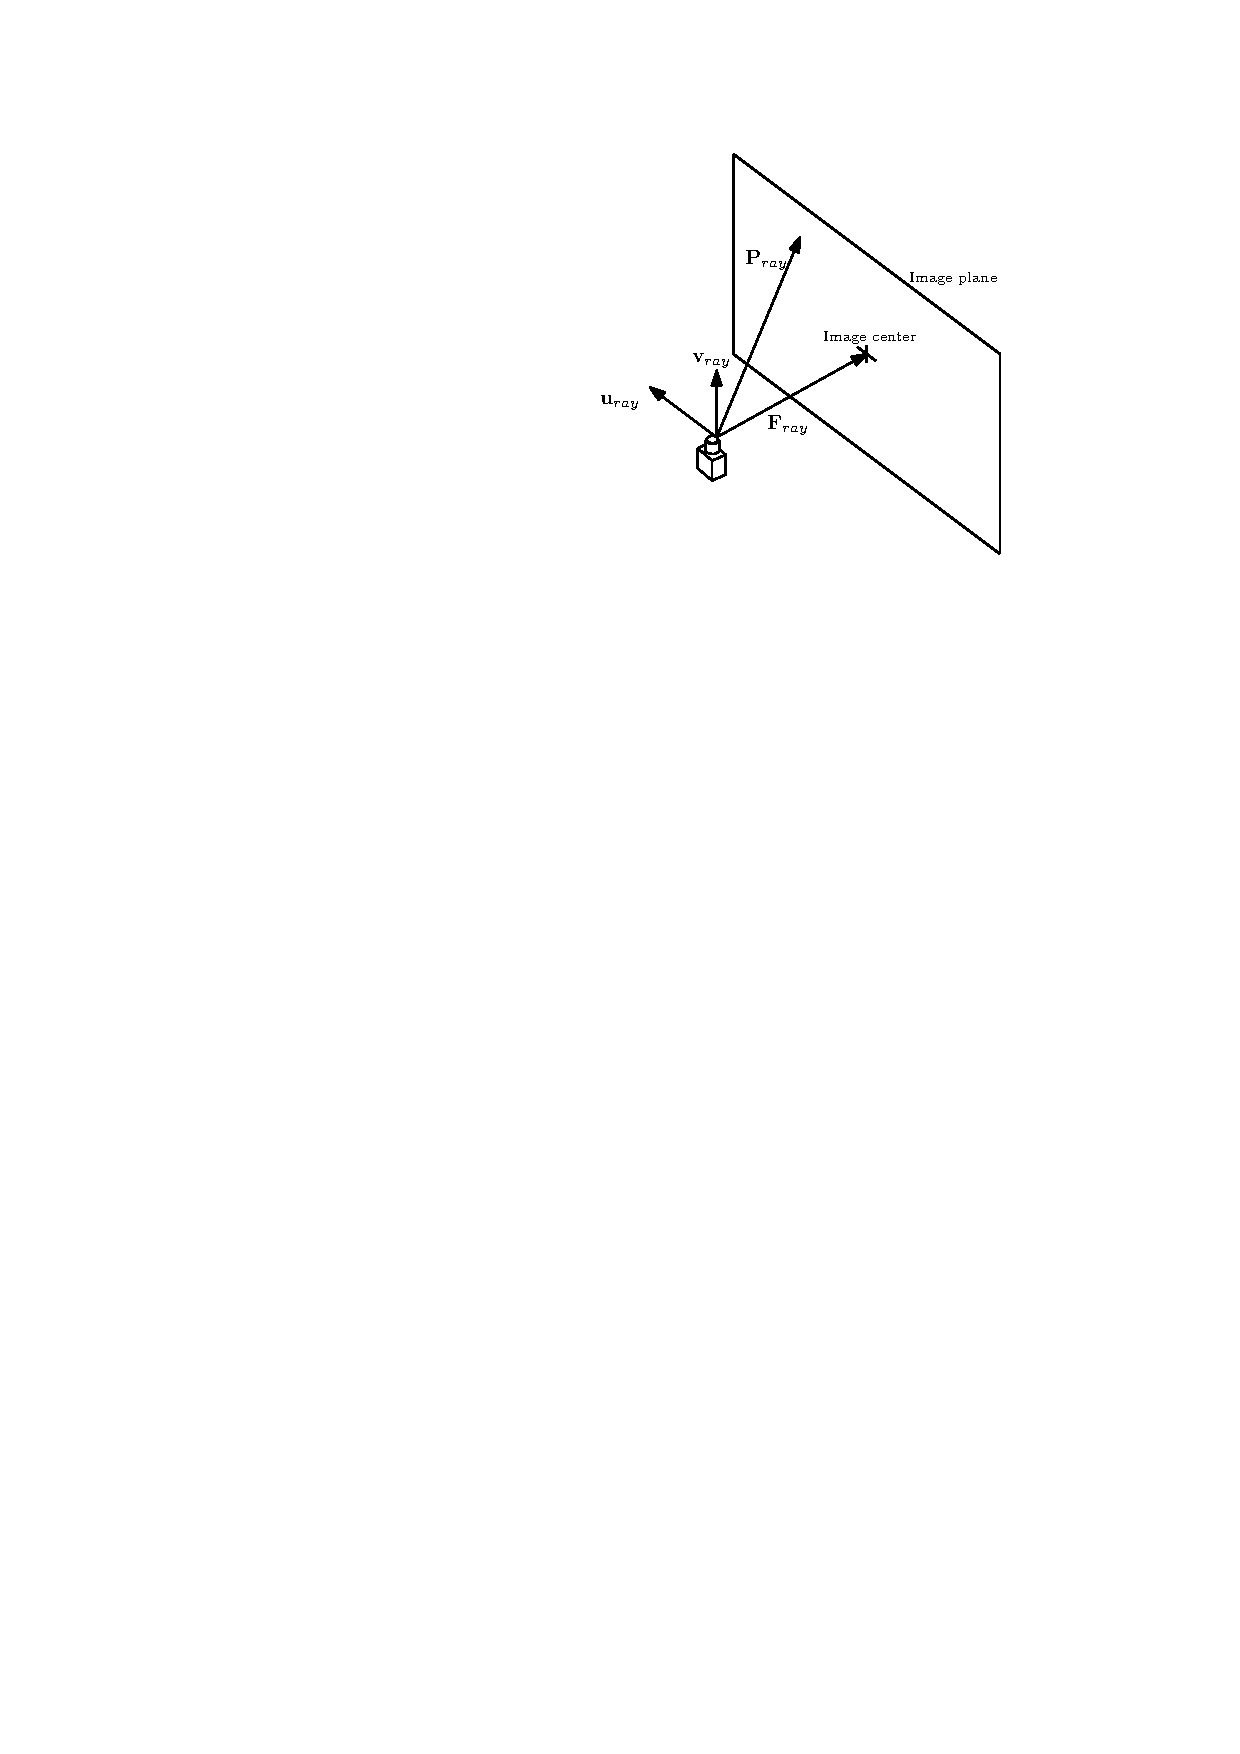
\includegraphics[width=0.5\textwidth]{chapters/images/omni_perspective}
  \caption{Defining rays on a desired image plane to form a perspective image}
  \label{fig:omni_perspective}
\end{figure}

The focal length will be the desired focal length of the new perspective image. This can be defined by the user.  The size of the perspective image $\bv I(cols, rows)$ may also be defined by the user.  The function project($\bv P$) takes a 3D ray $\bv P$ and projects it to 2D pixel coordinates.  The pixel coordinates returned will be represented as floating point variables.  Therefore, the function bilinearInterpolate($\bv P$)(cite) takes these pixel coordinates and produces an approximation of the intensity at these coordinates from the unwrapped image using bilinear interpolation.

In practice, the rays will be the same for a set of perspective image parameters.  Therefore the rays are pre-calculated in the form of a perspective pixel coordinate to omni pixel coordinate lookup table.

\begin{figure}[b!]
  \centering
    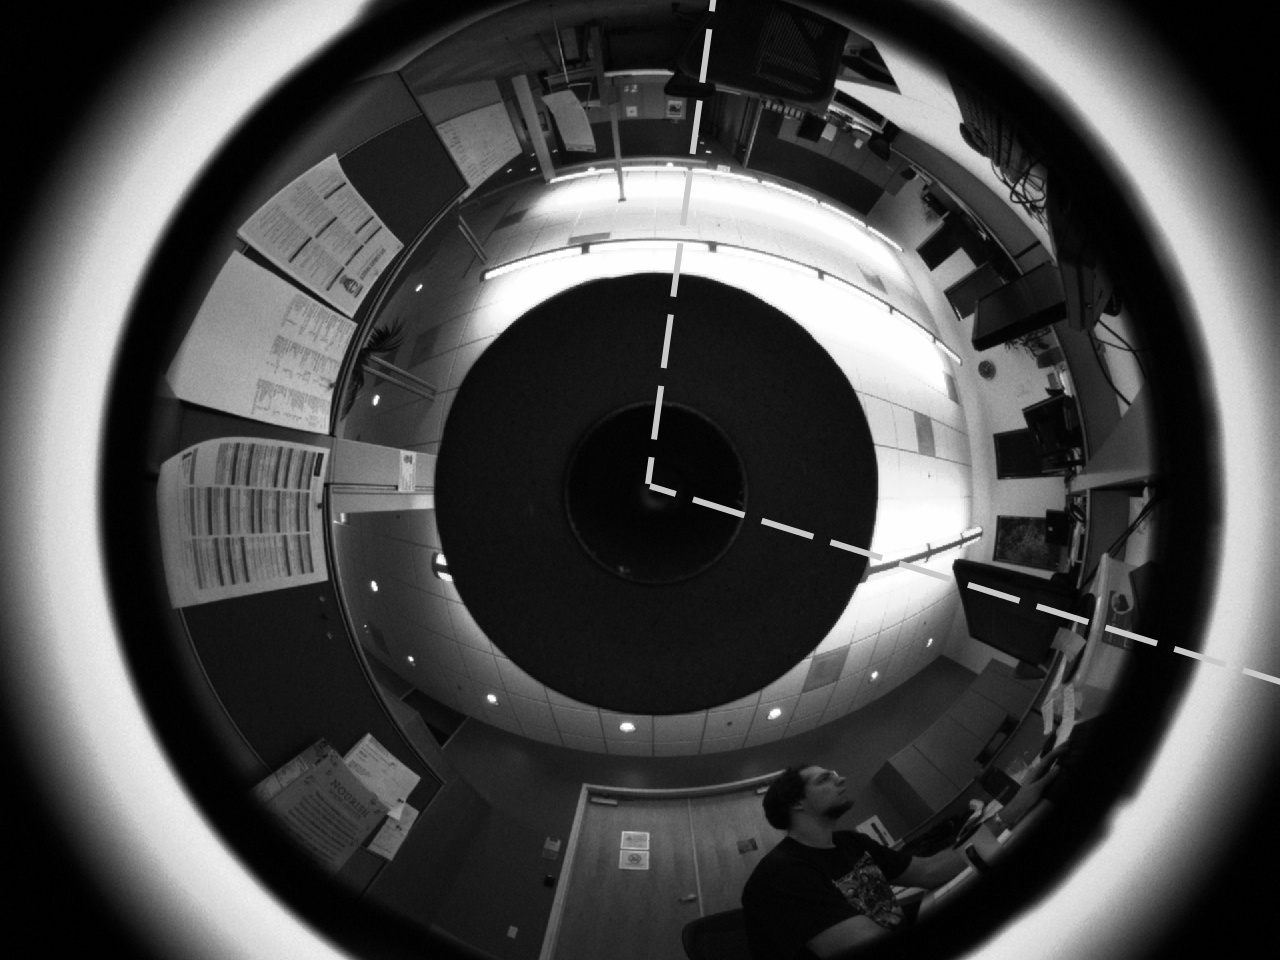
\includegraphics[width=0.32\textwidth]{chapters/images/omni_raw_office}
    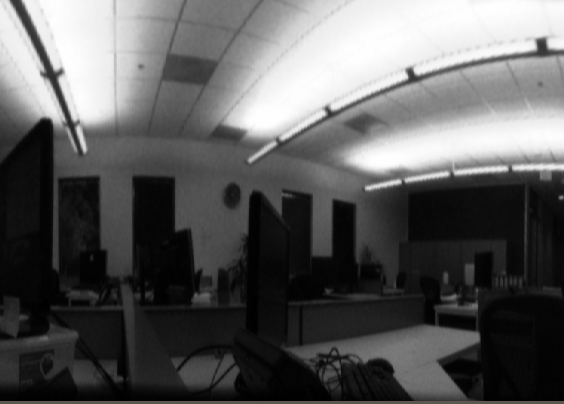
\includegraphics[width=0.32\textwidth]{chapters/images/unwrapped_office}
    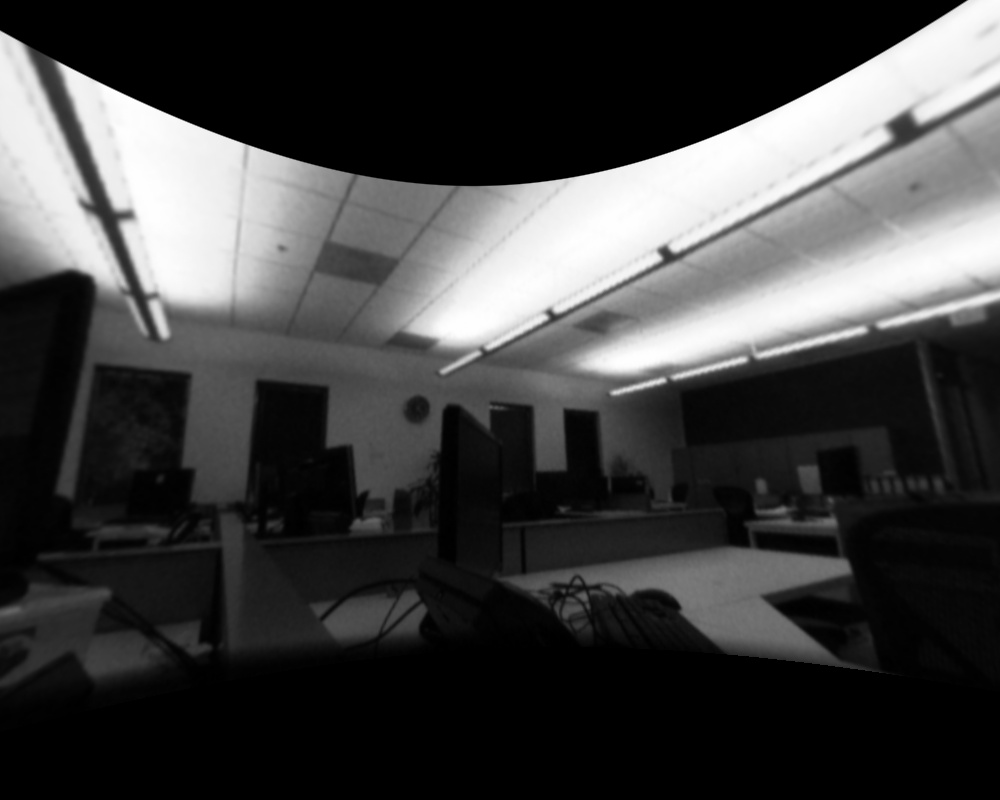
\includegraphics[width=0.32\textwidth]{chapters/images/perspective_office}
  \caption{Left: Original omni camera image with lines denoting a section.  Center: That particular section from the unwrapped image.  Right: Perspective image of the same section.  Note that all the lines are straight in the perspective image, whereas they are distorted in both the original omni and unwrapped image.}
  \label{fig:omni_images}
\end{figure}

The advantage of this algorithm is that the perspective image plane is very configurable.  It is possible to define image center direction, image plane orientation about the optical axis, resolution and focal length (which in turn defines field of view).  Therefore it is convenient, given that the omni camera is mounted near another camera to be calibrated against, to define an overlapping field of view with that other camera. %TODO long sentence

\section{Online validation of extrinsic calibration}
\label{sec:verification_tool}

Using the stereo camera, it is possible to verify the extrinsic calibration without the use of the checkerboard.  In this case, the baseline of the stereo camera determined from stereo calibration is assumed to be correct and utilised.  Points matched between left and right stereo frames may be triangulated to find their 3D positions.  These points can then be reprojected into the omni camera image using the extrinsic calibration.

\begin{figure}[h!]
  \centering
    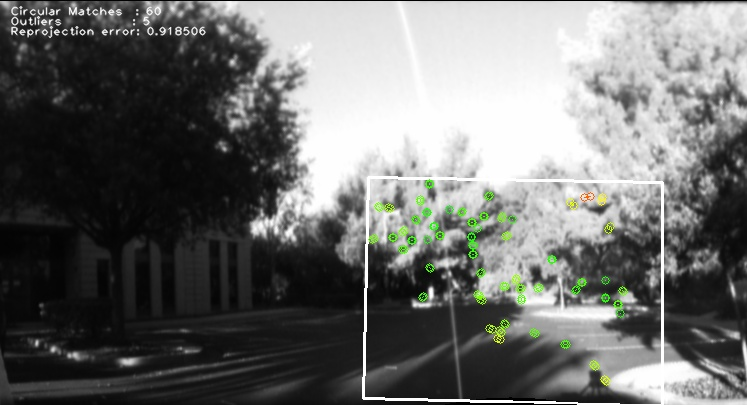
\includegraphics[width=1.0\textwidth]{chapters/images/circ_matches}
  \caption{Visualization of the extrinsic verification tool. This is a cropped image of the unwrapped omni image.  The white square represents the field of view of the stereo camera.  Stereo points have been reprojected into this image and overlayed onto the matching keypoints from the omni image. }
  \label{fig:circ_matches}
\end{figure}

A verification tool was developed to perform this operation.  Circular matching is done between left stereo frame, right stereo frame and the unwrapped omni image, to remove outliers.  Stereo matches are used to generate 3D points.  These points are transformed to the omni camera frame, and then projected into the image.  They are visualized with lines drawn to their corresponding match from the omni image.  Reprojection error over all points is calculated and also visualized.  This program can run online, at a frame rate of about 1-2Hz (low frame rate due to feature extraction and circular matching).  This is useful for verifying the extrinsic calibration and demonstrating online that omni/stereo matching is successful.

This tool also serves a second purpose; mainly to log all of the 2D omni points and corresponding 3D stereo points.  From this data, a second extrinsic refinement could be performed, by minimizing the reprojection error over all points.  This calibration uses the known geometry of the stereo camera as opposed to known geometry of the checkerboard.  This means that any feature matched in both stereo frames and omni camera frame can be used as a data point for calibration.

\section{Non linear extrinsic refinement}
\label{sec:g2o_extrinsic_cal}

In the setup used, the tool described in Secion \ref{sec:ros_tool} did not produce a satisfactory calibration; reprojection error was found to be as high as 12 pixels for valid matches.  The reason being is that the omni camera was mounted high above the stereo camera in order to maximise field of view.  However, this meant that the overlap of both images was minimal, particularly indoors, where there was not enough space to move the checkerboard to different positions.  Therefore not enough checkerboard measurements could be recorded in order to achieve an accurate calibration.

A simple g2o graph was implemented to perform the extrinsic refinement optimization as mentioned in Section \ref{sec:verification_tool}.  The 2D and 3D points are represented as fixed vertices.  The pose to transform from stereo to omni frame is an SE(3) pose, in this case, one of the inbuilt g2o types.  A single edge joins a 2D and 3D point, along with the SE(3) calibration vertex, and calculates the reprojection error as follows:

\begin{align}
 \bv e = \bv z_{OM} - \hat{\bv z}( ^{OM}\bv T_{ST} \bv P_{ST})
\end{align}

$\bv z_{OM}$ represents 2D pixel coordinates of a single point in the omni image and $\hat{\bv z}$ projects a 3D world point to a 2D image point.  $\bv P_{ST}$ is a 3D point in the stereo frame. Finally, $^{OM}\bv T_{ST}$, which transforms points from the stereo camera frame to omni camera frame, is the transformation to optimize over.  A 3D visualization of the non linear calibration can be seen in Fig. \ref{fig:g2o_cal_vis}

\begin{figure}[h!]
  \centering
    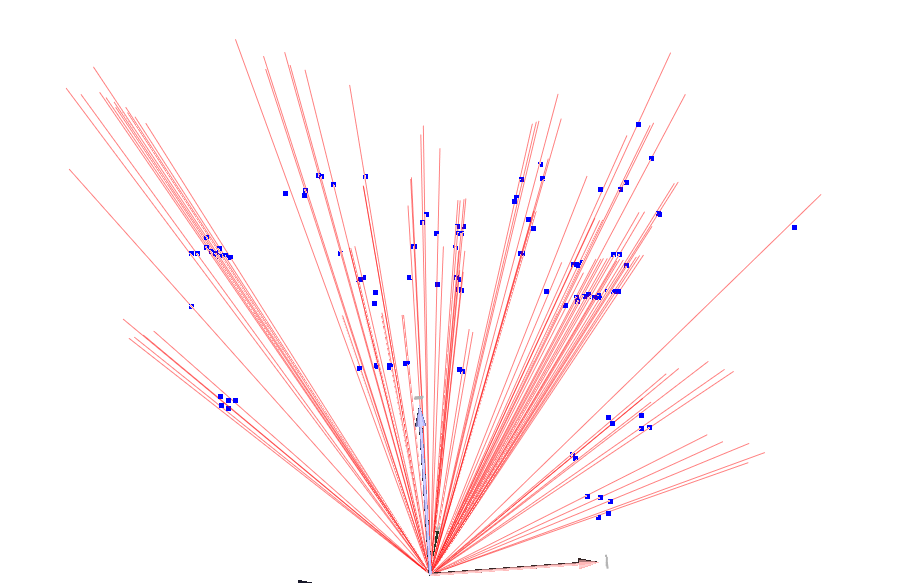
\includegraphics[width=0.7\textwidth]{chapters/images/g2o_cal_vis}
  \caption{3D visualization of the g2o non linear extrinsic optimization.  The rays represent features extracted from the omni image, and the points are 3D stereo points.  Ideally the rays should intersect through their corresponding points}
  \label{fig:g2o_cal_vis}
\end{figure}

To perform this calibration, data was collected using the online verfication tool.  An initial condition was obtained from the calibration produced from the tool mentioned in Section \ref{sec:ros_tool}.  After the non linear optimization converged, the new pose could be checked by the verfication tool.  A visualization of before and after optimization can be seen in Fig. \ref{fig:before_after_g2o}. 

An important factor discoverd when using this calibration tool was to have points over the whole image space, and also with a wide range of depth.  Initial calibrations showed excellent performance in terms of reprojection error on the data points used for calibration, however it was not stable for new points at different depths.  It was also noted that the geometry of the optimized pose was not representative of the real world pose between stereo and omni cameras.  

Tables \ref{tab:reprojection_error} and \ref{tab:geometry} show reprojection error results and the translation component of the pose between the cameras using data collected in different areas. 'Indoors' denotes the dataset collected when the vehicle was inside, where all points were close. 'Outdoors' denotes data collected outdoors, namely the scene depicted in Fig. \ref{fig:before_after_g2o}, where all points were far away.  'Both' denotes both datasets combined together for optimization.

For Table \ref{tab:geometry}, the rough measurement of the stereo camera position with respect to the omni camera reference frame was done with a ruler, and some axes were difficult to measure given the geometry of the test vehicle.  Therefore the accuracy is low, however it should be within about 10cm.

\begin{table}[H]
   \begin{tabular}{ p{6cm} r r }
    \toprule
    & \multicolumn{2}{r}{\bf{Average Reprojection error on dataset}}  \\
    & \multicolumn{1}{c}{\hspace*{2cm}\bf{Indoors}} & \multicolumn{1}{c}{\hspace*{2cm}\bf{Outside}} \\
    \midrule
    Optimized using Indoors  & 0.42  & 87.05 \\
    Optimized using Outdoors & 13.82 & 0.63 \\
    Optimized using Both     & 0.53  & 0.96 \\ 
    \bottomrule
    \end{tabular}
    \captionof{table} {Reprojection errors for extrinsic optimization using different datasets} 
  \label{tab:reprojection_error}
\end{table}

% original accuracy:
%Optimized using Indoors & 0.425 & 87.050 \\
%Optimized using Outdoors & 13.82 & 0.634 \\
%Optimized using Both & 0.533 & 0.968 \\ 

\begin{table}[H]
    \begin{tabular}{ p{6cm} r r r} % p{5cm} |}
    \toprule
    & \multicolumn{3}{r}{\bf{Translation component from pose}}  \\
    & \multicolumn{1}{c}{\hspace*{1cm}\bf{x (cm)}} & \multicolumn{1}{c}{\hspace*{1cm}\bf{y (cm)}} & \hspace*{1cm}\bf{z (cm)} \\
    \midrule
    Rough Measurement & 10.0 & -100.0 & -50.0 \\
    Optimized using Indoors & -36.4 & -85.0 & -18.5\\
    Optimized using Outdoors & 11.2 & 43.0 & -37.1 \\
    Optimized using Both & 13.0 & -92.5 & -46.9 \\ 
    \bottomrule
    \end{tabular}
    \captionof{table}{Translational component of the transformation that transforms points from the stereo camera frame to the omni camera frame}
  \label{tab:geometry}
\end{table}

Table \ref{tab:reprojection_error} shows that when only optimizing on indoors or outdoors datasets, the reprojection error was very high in the area not used for optimization.  It also shows very low reprojection error when optimizing using both datasets (less then 1.0 pixels).  This verifies that points over a wide range of distances is required for calibration, and it also shows an excellent overall calibration result.

Table \ref{tab:geometry} reflects the same result as Table \ref{tab:reprojection_error}.  The geometry of 'Indoors' and 'Outdoors' are quite clearly wrong.  Comparing the rough measurement with the optimization of both datasets, all values are within 10cm, which is expected.

These results show that a good calibration, both in terms of reprojection error and geometrical accuracy can be obtained by calibrating using data points over a wide range of depth. Details of the exact calibration procedure used for evaluation can be found in Section \ref{subsubsec:actual_calibation}.

\begin{figure}[h!]
  \centering
    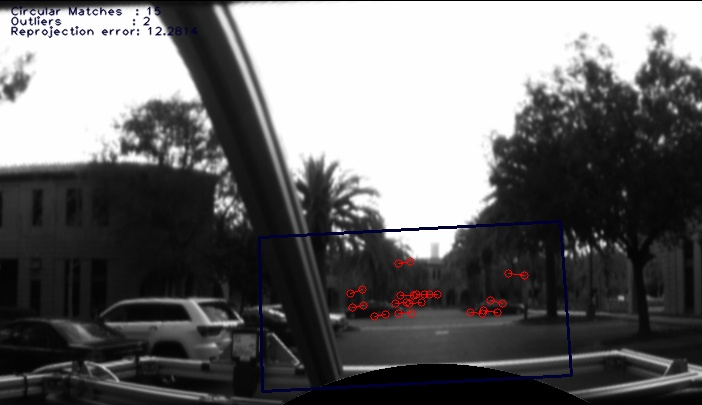
\includegraphics[width=1.0\textwidth]{chapters/images/verify_before_opt}
    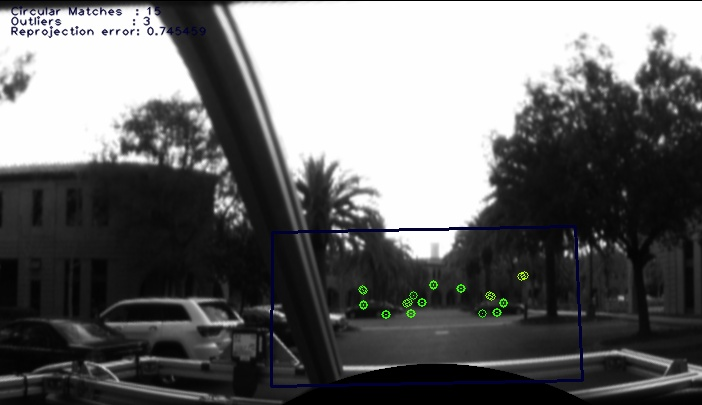
\includegraphics[width=1.0\textwidth]{chapters/images/verify_after_opt}
  \caption{Before and after non linear optimization of the extrinsic calibration.  In this example, the average reprojection error was reduced from 12.34 to 0.63}
  \label{fig:before_after_g2o}
\end{figure}